\section{Introduction}

% Multimodal Large Language Models (MLLMs) .

% In the field of Computer Science, 
Recently, with the emergence of Large Language Models (LLMs) such as GPT-4 \cite{openai2023gpt4}, the cognitive abilities of language models have reached a new level \cite{zhuang2023efficiently}.
They demonstrated remarkable performance in many tasks \cite{bubeck2023sparks}.
% \KZ{Citations and evidence of the above?} \XJ{Fixed}
% Many researchers try to enhance the Vision Language Pre-trained Models (VLPMs) by incorporating powerful LLMs, which are called large vision-language models (LVLMs). 
In Vision Language (VL), several researchers \cite{zhu2023minigpt, liu2023llava, ye2023mplug} endeavor to boost Vision Language Pre-trained Models (VLPMs) by integrating powerful LLMs \cite{touvron2023llama, chiang2023vicuna}, referred to as Large Vision-Language Models (LVLMs).
With LLM as the ``brain'', the cognitive abilities of LVLMs are also improved and more challenging tasks, such as table, chart, and document reasoning etc, can be solved \cite{yang2023dawn}. 
% \KZ{What are these tasks and how did LVLMs fare?} \XJ{Fixed}
Some state-of-the-art LVLMs, such as GPT-4V \cite{openai2023gpt4}, 
are progressing towards human-level cognitive abilities.
% \KZ{What is considered human-level cognition ability? How to measure one's cognition ability?}
% \XJ{Seems there's no strict quantitative calculation method, only qualitative analysis.}
% Thus, how to evaluate the cognitive ability of LVLMs becomes an important and urgent issue. 
% Thus, effectively evaluating the cognitive ability of LVLMs has become an increasingly important concern.
Thus, there's an increasing interset in evaluating the cognitive abilities of LVLMs.
Though some LVLM evaluation benchmarks, such as MME \cite{fu2023mme}, MMBench \cite{liu2023mmbench}, SEED Bench \cite{li2023seed}, etc., 
% \KZ{Name them and give cites}
% \XJ{fixed}
also consider cognitive reasoning ability as one aspect of their evaluation, they do not provide a comprehensive evaluation of higher-level reasoning ability via a concentrated task and most of the images they use require relatively little reasoning to understand. 
However with humans, we have such tasks like Cookie Theft picture description, which is broadly used to assess one's cognitive function. 
% rarely consider the cognitive reasoning ability demonstrated during the process of describing images.
% \KZ{I think u are being too
% brief here. These works are our competitors. You need to be more serious about
% them than just brushing them off.}
% \XJ{fixed}
% \KZ{If before this paper there's no definitive way to evaluate
% LVLM's cognitive abilities, then how can you say that recently LVLMs have
% already approached human level?}
% \XJ{cognitive abilities of models is usually measured by reasoning task. reference: from recognition to cognition: Visual Commonsense Reasoning.} 
% \MY{why do we care about LM's cognitive capability? just say that there's an increasing interset in such evaluation while they focus on certain aspects, lacking a comprehensive evaluation of higher-level ability, i.e. reasoning etc. via a concentrated task. However with humans, we have such tasks like picture description with cookie theft is broadly used to assess one's cognitive function.}

% \MY{We can also benefit from adding a citation of proper definition of cognitive function, to showcase that these abilities are not fully covered by current benchmarsk while they are essential to humans}z
% In cognitive function test with humans, Picture Description task is a common practice used to elicit spontaneous speech to aid in the diagnosis of diseases closely related to human language and cognitive functions, such as dementia.
% \MY{strictly speaking, dementia/cognitive dysfunction is not mental health, stick to cognitive function test with humans, or find formal sayings from moca introduction}
% \XJ{fixed}
% \KZ{The picture description task has been extenively used to diagose people with
% cognitive disorders such as dementia or Alzheimers disease, meaning it can be
% used to tell healthy, normal individuals from people who suffer from cognitive
% disorders. However, does this mean, better scores in such task means the person
% has more cognitive power?}
% \XJ{Maybe the premise for diagnosis is that there is a correlation between two variables?}
% It was found to be an effective speech task in evoking situations that required more cognitive effort \cite{JIANG201739}. 
Among different picture description tasks, the Cookie Theft picture description task (Figure \ref{fig:cookie_theft}) from the Boston Diagnostic Aphasia Examination \cite{goodglass2001-ej} has dominated work in speech-language pathology \cite{describe-ctp}. 
% Dementia Detection task can be performed based on descriptions elicited by the Cookie Theft picture.
Surprisingly, this picture has been developed and utilized for more than 50 years and continues to be applied and discussed today. 
% numerous studies have also been conducted based on the
% In Computer Science, researchers are performing Dementia Detection based on descriptions elicited by the Cookie Theft picture \cite{li-etal-2022-gpt, duan-etal-2023-cda, farzana-parde-2023-towards}. 
The success of Cookie Theft has sparked our curiosity to investigate the 
magic behind this picture and explore ways to apply this human-oriented 
cognitive ability assessment to evaluate cognitive abilities of LVLMs. 

% figure
\begin{figure}[th]
    \centering
    % 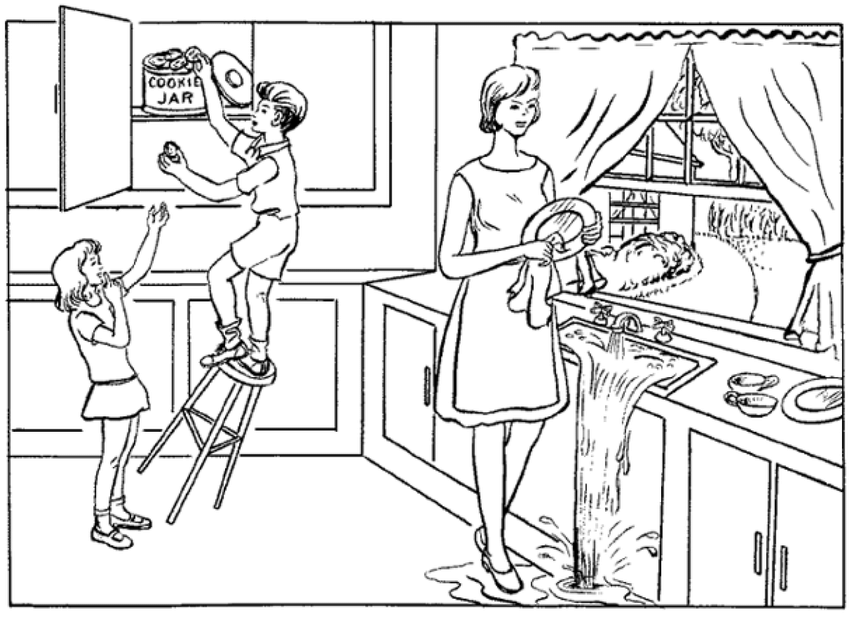
\includegraphics[width=0.4\textwidth]{figs/cookie_theft.png}
    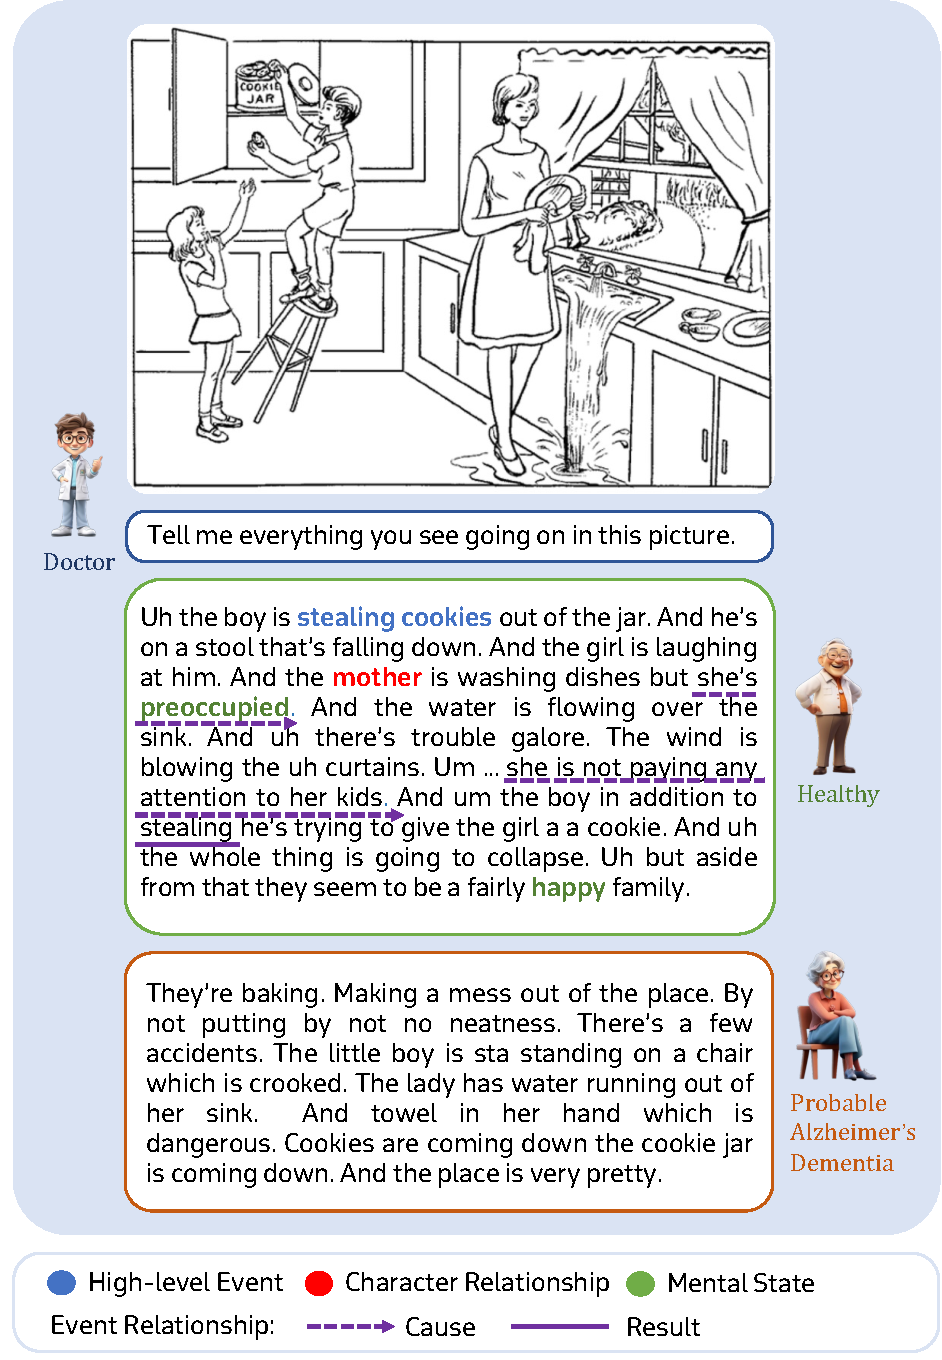
\includegraphics[width=0.45\textwidth]{figs/cookie_theft_description8.pdf}
    \caption{Cookie Theft picture description task. 
    % The description in the green frame was produced by a 75-year-old healthy man. 
    % The description in the orange frame was produced by an 66-year-old woman with probable Alzheimer's dementia. 
    The descriptions in the green frame and the orange frame were respectively produced by a 75-year-old healthy man and a 66-year-old woman with probable Alzheimer's dementia\protect\footnotemark. 
    % The healthy man's description demonstrates his cognitive ability by reasoning about different aspects, which is annotated in the description. 
    % \KZ{To me, the second description provided by the Alzheimers patient is not that bad!}
    % \XJ{fixed}
    % \KZ{The caption is too long-winded. The fonts are too small in this pic. Don't remove our comments without being sure to have fixed them!} 
    % \MY{agree, fonts are too small and caption is not appealing enough}
    % \XJ{fixed}
    }
    % \footnote{https://dementia.talkbank.org/}
    \label{fig:cookie_theft}
\end{figure}
\footnotetext{The two samples are extracted from DementiaBank (\url{https://dementia.talkbank.org/}), which records description transcripts from both healthy subjects and dementia patients.}

% Some studies suggest that due to the high sensitivity of the Cookie Theft picture in monitoring human language and cognitive abilities, 
\citet{describe-ctp} analyzed the reasons for the success of of Cookie Theft.
It was found that it contains information of varying degrees of salience and contains more semantic categories.
% More salient information is put at the core position of the picture and less salient information is put in the background. 
% It also contains more semantic categories, such as animate entities (``mother'' and ``girl''), inanimate entities (``window'' and ``plate''), abstract concepts (``the mother is daydreaming''), and concrete concepts (``the boy is falling'') etc. 
It was also found that during describing Cookie Theft, compared to individuals with cognitive impairments, healthy people tend to demonstrate their coginitive ability by reasoning.
% \KZ{Why do we have to use the analysis by Cummings to understand what's 
% important in this pic? Why don't we use the metric used by the psychiatrists
% who use this picture to do the diagnosis?}
% \XJ{Because there are no standardized assessment metrics, diferent people use it in different ways.}
% about character relationships, event relationships, mental states of subject, etc. 
% in the picture.
For instance, in Figure \ref{fig:cookie_theft}, by comparing the descriptions produced by the healthy man and the woman with probable Alzheimer's dementia, we can identify the following differences:
% compared with the description produced by a woman with probable Alzheimer's dementia, 
\begin{itemize}
	\item The description produced by a healthy man uses ``\textcolor{red}{mother}'' instead of ``lady'', indicating the reasoning about \textcolor{red}{character relationship}. 
	\item The healthy man used ``\textcolor{blue}{stealing cookies}'' instead of ``taking cookies'', indicating his reasoning about this \textcolor{blue}{high-level event}. 
    The description produced by the patient even did not mention this event at all. 
    \item The healthy man also used ``the mother is \textcolor{c2}{preoccupied}'' and ``\textcolor{c2}{happy}'' to describe people's \textcolor{c2}{mental state}. 
    % \MY{The green color of text is visually unfriendly, define RGB of the green, or use xcolor package and select something else.}
    \item The description also reflects the  \textcolor{c1}{causal relationships between events}.
    Because ``\textcolor{c1}{the mother is preoccupied}'' and ``\textcolor{c1}{not paying attention to her kids}'', ``\textcolor{c1}{kids are stealing cookies.}''
\end{itemize}
Through these reasoning processes, the difference of cognitive abilities between the two individuals is reflected in their descriptions. 
% \MY{this presentation of the contrast between healthy vs. patient is not clear, consider using bullet points or draw a figure to show the differences}

% causal and temporal relations and 
% created their own Cookie Theft-like picture and
Such a picture that can evaluate cognitive function is carefully designed and crafted.
\citet{tasnim-etal-2022-depac} introduced guidelines for drawing pictures similar to Cookie Theft, which is consistent with findings mentioned above.
% \KZ{I wonder if there's any follow-up work that aims to generate more of
% such pics?} 
% \XJ{seems no}% 
% This study generally shares consistent findings with the previous one.
% According to the guidlines, Cookie Theft-like pictures should depict familiar themes, have rich content and involve in relationships between components in the scene, etc.
%  (locations, objects, actions, ``dangerous'' elements, etc.)
% Besides, another notable feature of the Cookie Theft-like picture is its involvement in relationships between components in the scene.
% , such as character relationships, event relationships, etc.
Generally speaking, compared to typical images, Cookie Theft-like images feature a prominent story theme, richer content, display relationships between components and require stronger cognitive abilities to understand and describe.

% Thus, we propose to evaluate the cognitive ability of LVLMs with human oriented cognitive evaluation tasks like Cookie Theft picture description task.
% We believe this is both reasonable and necessary. 
% However, the semantic information contained in the images in existing datasets is not particularly rich. 
% \KZ{Instead of generating brand new pics, we opt to retrieve such pics from the web. But why we choose this route?} 
% \XJ{collecting can be seen as the first step for generating or automatically collecting.}% 
The above studies provided us with directions for collecting Cookie Theft-like images and developing assessment criteria to construct a cognitive evaluation benchmark, so that the idea of this human cognition assessment can be leveraged to evaluate cognition of LVLMs comprehensively.
% With the rapid development of model cognitive abilities, it is necessary to use methods closer to human cognitive assessment to evaluate LVLMs.
% which is design for human cognition evaluation.
To fill this research gap, we propose to construct a \textbf{Cog}nitive Evaluation \textbf{Bench}mark, named as CogBench, which consists of high quality Cookie Theft-like images to evaluate the cognitive reasoning ability of LVLMs. 
CogBench defines eight core cognitive reasoning capabilities, including reasoning about special time, location, character, character relationship, event, event relationship, next moment event and mental state. 
Both a generative Image Description task and a discriminative Visual Question Answering (VQA) task are designed.
% \MY{thought we discussed these? too many acronyms, just say description and question-answering}
% Most of the data consists of ordinary photos (e.g., a picture of a restaurant) with more detailed descriptions, such as ``table'' vs. ``a brown wooden table.'' 
% The images lack elements that involve reasoning about interpersonal relationships, event relationships, and psychological states. This implies the need for the emergence of higher-quality and more challenging tasks/datasets.

% In this paper, we construct CogBench to evaluate high-level. 

Our main contributions are as follows:

\begin{itemize}
	\item To the best of our knowledge, this is the first-of-its-kind
attempt to incorporate the cognitive test Cookie-Theft picture description task designed for humans into the evaluation 
of LVLMs.
    % \KZ{Don't use the word ``borrow''.}
    % \XJ{fixed}
    % First, we construct CogBench to assess the cognitive abilities of LVLMs. 
%    We propose to use a human-like image description task to comprehensively evaluate the higher-level cognitive abilities of LVLMs. 
    % \KZ{How do we know
    % that we are eval ``high level'' cognitive abilities. Previously there are other
    % VL tasks. How do we show that ours is any different from those?}
    % \XJ{As shown in Figure \ref{fig:cogbench_example}, our images contains more CoRs and require stronger cognitive capability to understand and describe.}
    % \MY{My original thought was citing psychological definition of cognition and higher-level cog ability encompasing chain of reasoning, then providing the fact that previous VL tasks lack such.}
    % We introduce the concept of Cookie Theft-like images and images in CogBench are carefully selected to meet the criteria of Cookie Theft as much as possible, which require stronger cognitive capability to understand and describe. 
    % \KZ{We created the first ever and the largest to-date image
    % description task and dataset to evaluate LLM's cognitive abilities.}
    % \XJ{fixed}
    % As far as we know, we are the first to evaluate the cognitive ability of LVLMs with human-oriented cognitive evaluation Cookie Theft picture description task.
	% that demands stronger cognitive capability from models, aiming
    %The benchmark consists of two tasks: a generative task Cognitive Image Description (CogID) and a descriminitive task Cognitive Visual Question Answering (CogVQA).
	\item 
%To transfer the Cookie Theft picture description task to the evaluation of LVLMs, 
We created the first ever and the largest to-date VL dataset with Cookie Theft-like 
images to evaluate LVLM's cognitive abilities. 
%    Images in our dataset require stronger cognitive capability to understand and describe.
%    Annotation of the images provides the foundation for our proposed image description task and an additional question-answering task for CogBench.
    % \KZ{If it only takes one pic to evaluate a human's cog ability, why do we need
    % to create so many pics to test the LVLMs? Again, how do we show that this 
    % dataset is any better than previous such LV datasets in terms of testing one's
    % cog ability?} \XJ{Because the cognitive tests are aimed at individuals experiencing cognitive decline. The model's cognitive tests are designed for models whose cognitive abilities are continuously advancing. added a figure in image collection section.}
    % By annotating collected images with entities, fine-grained Chain of Reasonings (CoRs) and description, we construct a high-quality and high-level image-text dataset and propose Cognitive Image Description (CogID) task to evaluate LVLM's cognitive abilities in a fine-grained manner. 
    % This is the first ever image description task considering cognitive reasoning ability. 
    % Based on CoRs, we propose a CoR-based GPT-assisted Question Generation (CGQG) method to generate questions for CogVQA task.
    
    % To comprehensively evaluate the cognitive abilities of LVLMs, a generative image description task CogID and a discriminative Multiple Choice Question Answering task CogVQA are designed. 
    % Given the CogID task differs from traditional image captioning tasks, we developed a tailored evaluation methodology specifically designed for it. 
    % \KZ{This is hardly a contribution.} 
    % \XJ{fixed}
	\item 
%Based on CogBench, we evaluate some existing LVLMs. 
Our evaluation on existing well-known LVLMs shows that there is still a large gap between the cognitive ability of LVLMs and human beings, indicating CogBench is a challenging evaluation benchmark.
	
    % \MY{3 contributions: task itself (human-like image description to comprehensively test higher-level capability), images as benchmark with a split of description and QA, evaluation results.}

\end{itemize}

